\documentclass[12pt]{article}
\usepackage[utf8]{inputenc}
\usepackage[greek,english]{babel}
\usepackage{graphicx}
\usepackage{fontspec}
\setmainfont{Times New Roman} % Μπορούσα και GFS Didot
\usepackage[a4paper, margin=2.5cm]{geometry}
\usepackage{setspace}
\onehalfspacing
\usepackage{titlesec}
\usepackage{titling}
\usepackage{fancyhdr}
\usepackage{amsmath}
\usepackage{array}
\usepackage{emptypage}
\usepackage{lipsum}
\usepackage{xcolor}
\usepackage{hyperref}



\selectlanguage{greek}

\begin{document}
\thispagestyle{empty}
\begin{center}
    
\includegraphics[width=0.185\textwidth]{images/ntua_logo.png} \\ % Make sure the logo image exists here
    \noindent\rule{0pt}{1.5em}


    \textbf{\Large ΕΘΝΙΚΟ ΜΕΤΣΟΒΙΟ ΠΟΛΥΤΕΧΝΕΙΟ} \\[0.5em]
    Σχολή Εφαρμοσμένων Μαθηματικών και Φυσικών Επιστημών \\[0.5em]
    Τομέας Μαθηματικών \\[3em]

\vspace{1.9cm} 

    {\selectlanguage{english}
    
    \textbf{\Large Panoptic Segmentation with Deep Neural Networks} \\[2em]
    }

    \textbf{\LARGE ΔΙΠΛΩΜΑΤΙΚΗ ΕΡΓΑΣΙΑ} \\[1.5em]

    του \\
    \textbf{Νικόλα Ιωάννου} \\[4em]

\vspace{1.8cm} 


\hspace*{-0.3cm}\textbf{Επιβλέπων:} Παναγιώτης Τσανάκας       \hspace*{3.65cm} \textbf{Συνεπιβλέπων:} Γεώργιος Σιόλας \\
\hspace*{1.76cm}Καθηγητής Ε.Μ.Π.  \hspace*{7.23cm}Ε.ΔΙ.Π. Ε.Μ.Π.

\vspace{5.5 cm} 






    \scalebox{0.9}{ΕΡΓΑΣΤΗΡΙΟ ΟΡΑΣΗΣ ΥΠΟΛΟΓΙΣΤΩΝ, ΕΠΙΚΟΙΝΩΝΙΑΣ ΛΟΓΟΥ ΚΑΙ ΕΠΕΞΕΡΓΑΣΙΑΣ ΣΗΜΑΤΩΝ} 
 \\
    \scalebox{1}{Αθήνα, Ιούλιος 2025}
\end{center}
\pagenumbering{roman}
\newpage
\mbox{}
\newpage

\begin{center}
\noindent
\begin{minipage}{0.2\textwidth}
    \hspace*{10pt} %
    
\includegraphics[width=2.8cm,height=2.8cm]{images/ntua_logo.png} % Adjust path if needed
\end{minipage}
\hfill
\begin{minipage}{0.75\textwidth}
    \selectlanguage{greek}
    \small % or \footnotesize or any other size you want
    \textbf{Εθνικό Μετσόβιο Πολυτεχνείο}\\[-2pt]
    Σχολή Εφαρμοσμένων Μαθηματικών και Φυσικών Επιστημών\\[-2pt]
    Τομέας Μαθηματικών\\[-2pt]
    Εργαστήριο Όρασης Υπολογιστών, Επικοινωνίας Λόγου και Επεξεργασίας Σημάτων
\end{minipage}


\vspace{2.5cm} 

    {\selectlanguage{english}
    
    \textbf{\Large Panoptic Segmentation with Deep Neural Networks} \\[2em]
    }

    \textbf{\LARGE ΔΙΠΛΩΜΑΤΙΚΗ ΕΡΓΑΣΙΑ} \\[1.5em]

    του \\
    \textbf{Νικόλα Ιωάννου} \\[4em]

\vspace{0.6cm} 


\hspace*{-0.3cm}\textbf{Επιβλέπων:} Παναγιώτης Τσανάκας       \hspace*{3.65cm} \textbf{Συνεπιβλέπων:} Γεώργιος Σιόλας \\
\hspace*{1.76cm}Καθηγητής Ε.Μ.Π.  \hspace*{7.23cm}Ε.ΔΙ.Π. Ε.Μ.Π.

\vspace{2.5cm}
{\raggedright \small Εγκρίθηκε από την τριμελή εξεταστική
 επιτροπή την 1η Ιουλίου, 2025. \\
 
 }

\vspace{2cm}

(Υπογραφή)\hspace*{4cm} (Υπογραφή)\hspace*{4cm} (Υπογραφή)\\
\vspace{0.8 cm} 
.................... \hspace*{4cm} ....................\hspace*{4cm}  ....................\\
Παναγιώτης Τσανάκας\hspace*{2.4cm}  Αντώνιος Συμβώνης\hspace*{3cm}  Γεώργιος Στάμου \\
 Καθηγητής Ε.Μ.Π.\hspace*{3cm} 	 Καθηγητής Ε.Μ.Π.\hspace*{3cm}  Καθηγητής Ε.Μ.Π. 


\vspace{2.9 cm} 






    \scalebox{1}{Αθήνα, Ιούλιος 2025}
\end{center}

\newpage

\vspace*{\fill}
	{\raggedleft ........................................\\
    \textbf ΙΩΑΝΝΟΥ ΝΙΚΟΛΑΣ\\
    \textit{Διπλωματούχος σχολής Εφαρμοσμένων\\
    Μαθηματικών και Φυσικών Επιστημών Ε.Μ.Π.}
    
    }

\vspace*{\fill}


\vspace{2cm}
{
\small
\noindent \textcolor{black}{\textcopyright{} -- All rights reserved. Με επιφύλαξη παντός δικαιώματος.\\ Νικόλας Ιωάννου, 2025.}\\


\vspace{0.1cm}


\noindent\textcolor{black}{ Απαγορεύεται η αντιγραφή, αποθήκευση και διανομή της παρούσας εργασίας, εξ ολοκλήρου ή τμήματος αυτής, για
εμπορικούς σκοπούς. Επιτρέπεται η ανατύπωση, αποθήκευση και διανομή για σκοπούς μη κερδοσκοπικούς, εκπαιδευτικής
ή ερευνητικής φύσης, υπό την προϋπόθεση να αναφέρεται η πηγή προέλευσης και να διατηρείται το παρόν μήνυμα. Ερωτήματα που αφορούν τη χρήση της εργασίας για κερδοσκοπικό σκοπό πρέπει να απευθύνονται προς τον
συγγραφέα.
}

\vspace{0.1cm}

\noindent \textcolor{black}{ Οι απόψεις και τα συμπεράσματα που περιέχονται σε αυτό το έγγραφο εκφράζουν τον συγγραφέα και δεν πρέπει
να ερμηνευθεί ότι αντιπροσωπεύουν τις επίσημες θέσεις του Εθνικού Μετσόβιου Πολυτεχνείου.}}

\newpage
\mbox{}
\newpage

\section*{Περίληψη}
Στην


\newpage
\mbox{}
\newpage

\section*{Abstract}
in



\newpage
\mbox{}
\newpage

\section*{Ευχαριστίες}
Θα ήθελα να ευχαριστήσω τον κ.Παναγιώτη Τσανάκα για την επίβλεψη της παρούσας διπλωματικής εργασίας, όπως και τον κ.Γεώργιο Σιόλα για την καθοδήγηση και την συνεργασία την οποία είχαμε. Τέλος, θα ήθελα να ευχαριστήσω την οικογένεια μου γιατί χωρίς αυτούς δεν θα μπορούσα να βρίσκομαι στην θέση την οποία βρίσκομαι τώρα.


\newpage
\mbox{}
\newpage


\tableofcontents

\newpage
\listoffigures
\addcontentsline{toc}{part}{List of Figures}

\newpage
\listoftables
\addcontentsline{toc}{part}{List of Tables}

\newpage
\pagenumbering{arabic}
\section{Μαθηματικό υπόβαθρο}

\section{Εισαγωγή}

Η όραση υπολογιστών αποτελεί πεδίο της επιστήμης των υπολογιστών και της τεχνητής νοημοσύνης που εστιάζει στον εντοπισμό και την κατανόηση αντικειμένων σε ψηφιακές εικόνες και βίντεο απο υπολογιστές. Συγκεκριμένα, το πεδίο αυτό επιχειρεί να αναπαράγει αλγοριθμικά την αίσθηση της όρασης. Διαιρείται σε κατηγορίες με κάποιες απο τις κυριότερες εξ'αυτών να είναι: 

\begin{itemize}
    \item Εκτίμηση πόζας (Pose Estimation)
    \item Ανίχνευση αντικειμένων (Object Detection)
    \item Κατάτμηση εικόνας (Image Segmentation)
    \item Αναγνώριση προσώπου (Face recognition)
\end{itemize}

Η όραση υπολογιστών μπορεί να χρησιμοποιηθεί σε μια ευρύα γκάμα περιπτώσεων όπως στην ιατρική για τον εντοπισμό κακοήθη όγκου, στην αυτόνομη οδήγηση για τον εντοπισμό αντικειμένων και στην ρομποτική. \\

Η ιστορική της πορεία ξεκινά στις αρχές της δεκαετίας του 1950 με την έρευνα να επικεντρώνεται στην αναγνώριση απλών σχημάτων και μοτίβων μέσω ψηφιοποιημένων εικόνων. Ένα απο τα πρώτα σημεία αναφοράς του πεδίου ήταν το Summer Vision Project του ΜΙΤ το 1966, όπου ανατέθηκε σε φοιτητές να αναπτύξουν ένα ολοκληρωμένο σύστημα υπολογιστικής όρασης σε ένα καλοκαίρι. Αυτό βασίζεται στην τότε αντίληψη πως το πρόβλημα της υπολογιστικής όρασης πως αποτελεί ένα σχετικά απλό πρόβλημα. Κατά την δεκαετία του 1970, οι ερευνητές άρχισαν να διαμορφώνουν τα θεωρητικά θεμέλια της υπολογιστικής όρασης, όπως η ανίχνευση ακμών και η ανακατασκευή τρισδιάστατων σκηνών απο δύο διαστάσεις. Στη δεκαετία του 1980 η έρευνα μετατοπίστηκε απο την θεωρία στην πράξη με την ανάπτυξη τεχνικών που βασίζονταν κυρίως σε γραμμικά φίλτρα και μετασχηματισμούς (Hough και ο Fourier). Η δεκαετία του 1990 χαρακτηρίστικε με την αύξηση της υπολογιστικής ισχύος σε στροφή σε στατιστικές προσεγκίσεις και χρήση αλγορίθμων μηχανικής μάθησης. Η δεκαετία του 2010

\subsection{Κατάτμηση εικόνας}

Η κατάτμηση εικόνας αποτελεί τεχνική στην υπολογιστική όραση όπου μια ψηφιακή εικόνα διαιρείτε σε διακριτές περιοχές, με σκοπό τον εντοπισμό αντικειμένων στην εικόνα. Πιο συγκεκριμένα, η κατάτμηση εικόνας αποτελεί την διαδικασία κατά την οποία ανάλογα με την περίπτωση μερικά ή όλα τα εικονοστοιχεία της εικόνας ανατίθενται σε κλάσεις οι οποίες καθορίζουν το αντικείμενο. Η κατάτμηση εικόνας διαιρείται σε κατηγορίες με τις πιο κύριες εξ'αυτών να είναι:

\begin{itemize}
    \item Σημασιολογική κατάτμηση εικόνας
    \item Κατάτμηση παραδειγμάτων
    \item Πανοπτική κατάτμηση εικόνας
\end{itemize}

\subsubsection{Σημασιολογική κατάτμηση εικόνας}

Η σημασιολογική κατάτμηση εικόνας αποτελεί τεχνική κατά την οποία σε κάθε εικονοστοιχείο ανατίθεται μια κλάση. Στην τεχνική αυτή δεν γίνεται διαχωρισμός των διαφορετικών στοιχείων της ίδιας κλάσης. Για παράδειγμα, εάν σε μια εικόνα υπάρχουν 2 ανθρώποι, ο αλγόριθμος δεν θα τους διαχωρίσει ώς διαφορετικά αντικείμενα.

\begin{figure}[h!]
  \centering
  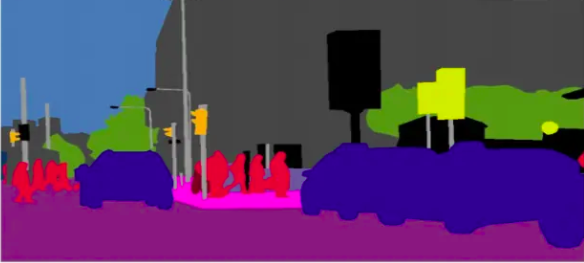
\includegraphics[width=0.6\textwidth]{images/figure1.png} % replace with your image file name
  \caption{Σημασιολογική κατάτμηση εικόνας}
  \label{figure 1}
\end{figure}

Όπως μπορούμε να δούμε στην \hyperref[figure 1]{εικόνα}, τα τρία αυτοκίνητα που παρουσιάζονται αναπαριστόνται με το ίδιο χρώμα, επιβεβαιώνοντας έτσι τα όσα αναφέρθηκαν παραπάνω. Επίσης, μπορούμε να παρατηρήσουμε πως δεν υπάρχει εικονοστοιχείο το οποίο να μην αντιστοιχήστηκε σε κάποια κλάση. \\

Κάποιες σημαντικές μετρικές απόδοσης της σημασιολογικής κατάτμησης εικόνας είναι η Intersection over Union (IoU), όπως επίσης και η Pixel Accuracy (PA). Μερικά παραδείγματα σημείων αναφοράς (benchmarks) για την μέτρηση της απόδοσης συγκεκριμένων αλγορίθμων που χρησιμοποιούν την τεχνική αυτή είναι τα Cityscapes, PASCAL VOC και ADE20K.

\subsubsection{Κατάτμηση παραδειγμάτων}
Η κατάτμηση παραδειγμάτων αποτελεί τεχνική κατά την οποία στα μόνο στα εικονοστοιχεία τα οποία αναπαριστούν κάποιο αντικείμενο ανατίθονται κλάση. Στην τεχνική αυτή σε αντίθεση με την σημασιολογική κατάτμηση εικόνας, γίνετε διαχωρισμός των διαφορετικών στοιχείων της ίδιας κλάσης. Για παράδειγμα χρησιμοποιώντας το παράδειγμα που αναφέραμε πρίν εάν σε μια εικόνα υπάρχουν περισσότεροι απο 1 ανθρώποι, ο αλγόριθμος θα διαχωρίσει κάθε εάν εξ'αυτών ώς διαφορετικά αντικείμενα(π.χ. Άνθρωπος 1, Άνθρωπος 2 κ.ο.κ.).

\begin{figure}[h!]
  \centering
  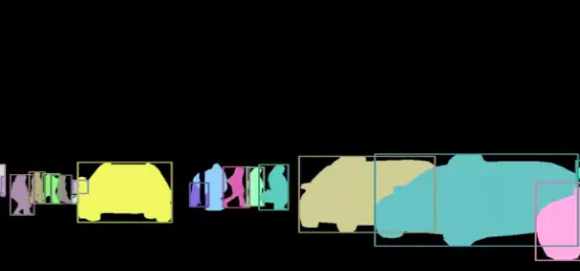
\includegraphics[width=0.6\textwidth]{images/figure2.png} % replace with your image file name
  \caption{Κατάτμηση παραδειγμάτων}
  \label{figure 2}
\end{figure}

\newpage
Όπως μπορούμε να δούμε στην εικόνα παραπάνω ο αλγόριθμος κατηγοριοποιεί μόνο τα εικονοστοιχεία τα οποία αντιστοιχούν σε κάποιο αντικείμενο, αδιαφορώντας για τα υπόλοιπα. Εύκολα μπορούμε να παρατηρήσουμε πως κατηγοριοποιούνται μόνο τα αυτοκίνητα και οι ανθρώποι, διακρίνωντας το κάθε αντικείμενο απο το άλλο, ανεξάρτητα εάν ανήκουν στην ίδια κλάση ή όχι. \\

Κάποιες σημαντικές μετρικές απόδοσης της κατάτμησης παραδείγματος είναι οι Average Precision (AP) και Mask Average Precision (Mask AP). Μερικά παραδείγματα σημείων αναφοράς γθα την μέτρηση της απόδοσης συγκεκριμένων αλγορίθμων που χρησιμοποιούν την τεχνική αυτή είναι τα COCO, Cityscapes και ADE20K.

\subsubsection{Πανοπτική κατάτμηση εικόνας}

Η πανοπτική κατάτμηση εικόνας αποτελεί την διαδικασία της ένωσης τον δύο προηγούμενων διαδικασιών. Πιο συγκεκριμένα, η τεχνική αυτή 

\begin{figure}[h!]
  \centering
  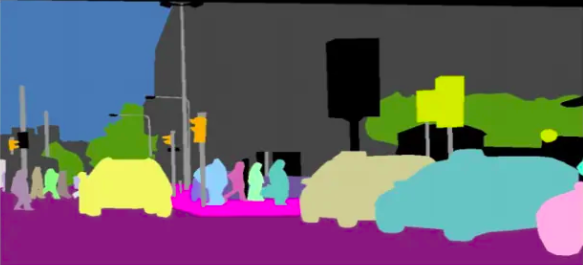
\includegraphics[width=0.6\textwidth]{images/figure3.png} % replace with your image file name
  \caption{Πανοπτική κατάτμηση εικόνας}
  \label{figure 3}
\end{figure}

\subsection{Σύνολα δεδομένων}

\subsection{Θεωρητικό υπόβαθρο}

\end{document}
